\documentclass[aspectratio=169,12pt]{beamer}

% Theme
\usetheme{Madrid}
\usecolortheme{default}
\setbeamertemplate{navigation symbols}{}
\setbeamertemplate{footline}[frame number]

% Packages
\usepackage[utf8]{inputenc}
\usepackage[T1]{fontenc}
\usepackage{amsmath,amssymb}
\usepackage{graphicx}
\usepackage{booktabs}
\usepackage{multirow}
\usepackage{array}
\usepackage{tikz}
\usepackage{appendixnumberbeamer}

% Colors
\definecolor{wur}{RGB}{0,100,50}
\definecolor{best}{RGB}{0,100,50}
\setbeamercolor{structure}{fg=wur}
\setbeamercolor{title}{fg=white,bg=wur}
\setbeamercolor{frametitle}{fg=white,bg=wur}

% Path to figures
\graphicspath{{../../3_Outputs/}}

% Shorthand
\newcommand{\eur}{\texteuro}
\newcommand{\best}[1]{\textcolor{best}{\textbf{#1}}}

% ============================================================
\title[Wheat Minimum Price Contract]{Extension: Minimum Price Contract \\for Wheat Output}
\subtitle{Progress Update --- AgEnRes Deliverable 5.4}
\author{Riccardo Spada}
\institute{Business Economics Group \\ Wageningen University \& Research}
\date{\today}

\begin{document}

% ============================================================
% TITLE
% ============================================================
\begin{frame}
\titlepage
\end{frame}

% ============================================================
% OUTLINE
% ============================================================
\begin{frame}{Outline}
\tableofcontents
\end{frame}

% ============================================================
% 1. RECAP
% ============================================================
\section{Recap: Input Price Risk}

\begin{frame}{Previous Work: Fertilizer Max-Price Contract}
\begin{itemize}
    \item European \textbf{call option} on CAN fertilizer price
    \item Farmer pays premium $\rho$; if spot price exceeds strike $K$, excess is covered
    \item Effective price paid: $\min(p_x^s,\, K) + \rho$
\end{itemize}

\vspace{0.5em}
\textbf{Key finding:}
\begin{itemize}
    \item Input price risk has a \textbf{limited impact} on total profit variability
    \item Profit variability mainly driven by \textbf{output prices and yields}
    \item[$\rightarrow$] Need to also address \textbf{output price risk}
\end{itemize}
\end{frame}

% ============================================================
% 2. EXTENSION
% ============================================================
\section{Extension: Wheat Minimum Price Contract}

\begin{frame}{New: Wheat Minimum Price Contract (Put Option)}
\begin{block}{Idea}
Add a \textbf{price floor} on wheat revenue using a European put option --- symmetric to the fertilizer price ceiling.
\end{block}

\vspace{0.5em}
\begin{itemize}
    \item Farmer pays premium $\rho_w$; if wheat spot price falls below strike $K_w$, the shortfall is covered
    \item Effective price received: $\max(p_w^s,\, K_w) - \rho_w$
    \item Addresses \textbf{downside output price risk} (revenue protection)
\end{itemize}

\vspace{0.5em}
\textbf{Additionally:} Evaluate a \textbf{combined contract} (fertilizer ceiling + wheat floor) to address both input and output risk simultaneously.
\end{frame}

\begin{frame}{Contract Design: Full Comparison}
\begin{table}
\centering
\small
\begin{tabular}{lccc}
\toprule
 & \textbf{Fertilizer call} & \textbf{Wheat put} & \textbf{Combined} \\
\midrule
Type & Call option & Put option & Call + Put \\
Risk hedged & Input cost $\uparrow$ & Revenue $\downarrow$ & Both \\
Effective price & $\min(p_x^s, K_f)$ & $\max(p_w^s, K_w)$ & Both \\
Premium & $\rho_f$ (\eur/kg) & $\rho_w$ (\eur/t) & $\rho_f + \rho_w$ \\
Premium (per ha) & $\rho_f \times \text{CAN}$ & $\rho_w \times y$ & sum \\
\midrule
Strike quantiles & 50th--90th & 10th--50th & Diagonal pairing \\
Maturity & 6 months & 12 months & Both \\
\bottomrule
\end{tabular}
\end{table}

\vspace{0.3em}
\small \textbf{Diagonal pairing:} fertilizer strike $i$ is paired with wheat strike $i$ (rank-matched).
\end{frame}

% ============================================================
% 3. PAYOFF STRUCTURE
% ============================================================
\section{Contract Payoff Structure}

\begin{frame}{Payoff Diagrams}
\begin{columns}[T]
\column{0.48\textwidth}
\textbf{Fertilizer: Price Ceiling (Call)}
\begin{figure}
    \centering
    \includegraphics[width=\textwidth]{ContractPayoffDiagram.pdf}
\end{figure}
Effective price \textbf{paid}: $\min(p_x^s, K_f)$

\column{0.48\textwidth}
\textbf{Wheat: Price Floor (Put)}
\begin{figure}
    \centering
    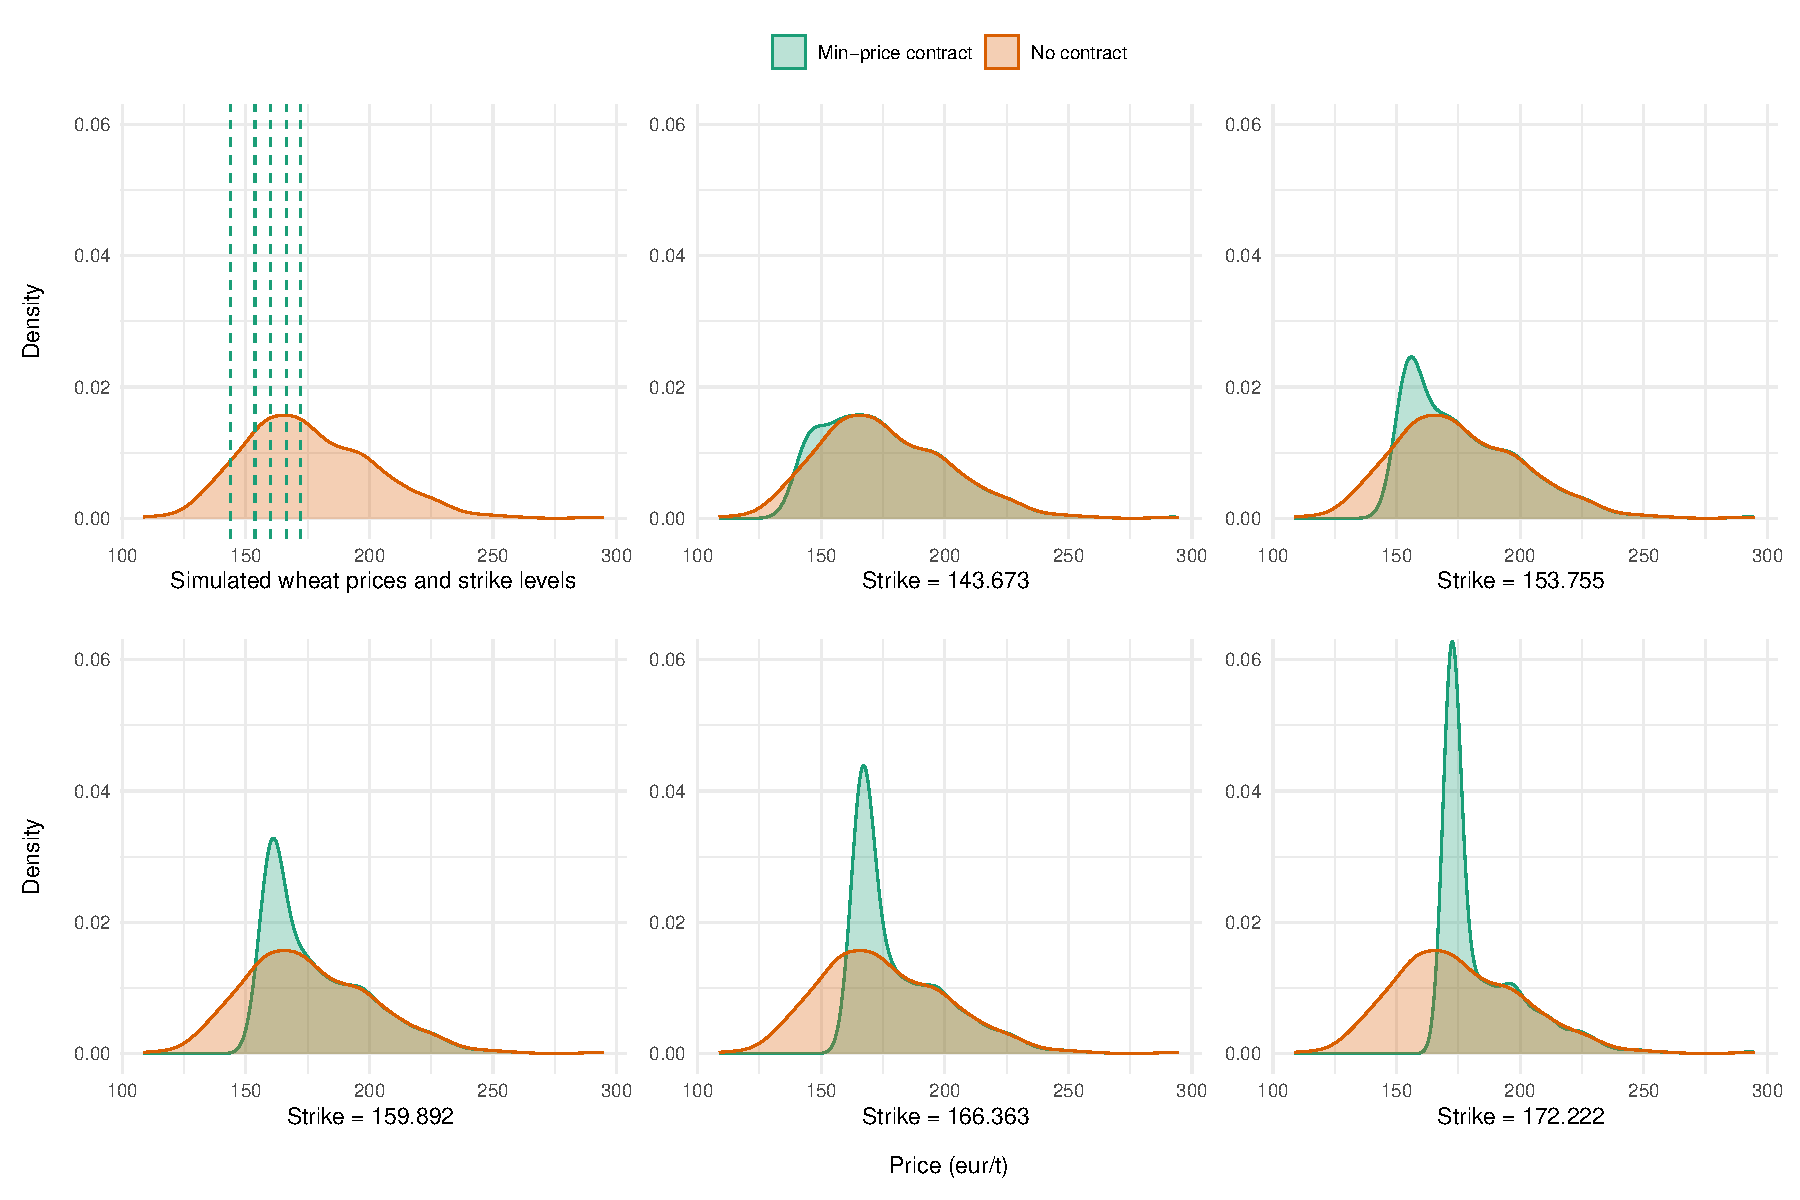
\includegraphics[width=\textwidth]{Fig_PriceDensities_SimulatedStrikes_Wheat.pdf}
\end{figure}
Effective price \textbf{received}: $\max(p_w^s, K_w)$
\end{columns}
\end{frame}

% ============================================================
% 4. CONTRACT PRICING
% ============================================================
\section{Contract Pricing}

\begin{frame}{Contract Pricing: Fertilizer Call vs.\ Wheat Put}
\begin{columns}[T]
\column{0.45\textwidth}
\textbf{Fertilizer call option}
\begin{table}
\centering
\small
\begin{tabular}{ccc}
\toprule
Quantile & Strike & Premium \\
 & (\eur/kg) & (\eur/kg) \\
\midrule
0.5 & 0.355 & 0.011 \\
0.6 & 0.361 & 0.008 \\
0.7 & 0.368 & 0.005 \\
0.8 & 0.376 & 0.004 \\
0.9 & 0.388 & 0.002 \\
\bottomrule
\end{tabular}
\end{table}
Higher strike $\rightarrow$ lower premium

\column{0.45\textwidth}
\textbf{Wheat put option}
\begin{table}
\centering
\small
\begin{tabular}{ccc}
\toprule
Quantile & Strike & Premium \\
 & (\eur/t) & (\eur/t) \\
\midrule
0.1 & 130.81 & 0.82 \\
0.2 & 138.80 & 1.95 \\
0.3 & 145.64 & 3.60 \\
0.4 & 151.92 & 5.75 \\
0.5 & 157.89 & 8.33 \\
\bottomrule
\end{tabular}
\end{table}
Higher strike $\rightarrow$ higher premium
\end{columns}

\vspace{0.5em}
\small Wheat put premiums are larger in absolute terms but small relative to wheat prices (0.5--5.3\% of strike).
\end{frame}

% ============================================================
% 5. PROFIT SCENARIOS
% ============================================================
\section{Profit Summary}

\begin{frame}{17 Profit Scenarios}
\small
\begin{table}
\centering
\begin{tabular}{lll}
\toprule
\textbf{Label} & \textbf{Contract} & \textbf{Profit formula} \\
\midrule
nc & No contract & $p_w^s \cdot y - p_x^s \cdot \text{CAN}$ \\
fc & Forward (fertilizer) & $p_w^s \cdot y - p_x^f \cdot \text{CAN}$ \\
\midrule
ac\_1\ldots5 & Fert.\ ceiling only & $p_w^s \cdot y - [\min(p_x^s, K_f) + \rho_f] \cdot \text{CAN}$ \\
wc\_1\ldots5 & Wheat floor only & $[\max(p_w^s, K_w) - \rho_w] \cdot y - p_x^s \cdot \text{CAN}$ \\
both\_1\ldots5 & Combined (diagonal) & $[\max(p_w^s, K_w) - \rho_w] \cdot y - [\min(p_x^s, K_f) + \rho_f] \cdot \text{CAN}$ \\
\bottomrule
\end{tabular}
\end{table}

\vspace{0.3em}
\begin{itemize}
    \item All evaluated under \textbf{1,000 simulated price paths} (copula-linked)
    \item EUT and CPT applied to all 17 columns automatically
    \item Broad framing: ref = $E[\pi^{fc}]$ \quad | \quad Narrow framing: ref = 0
\end{itemize}
\end{frame}

\begin{frame}{Profit Summary Statistics (\eur/ha)}
\footnotesize
\begin{table}
\centering
\resizebox{\textwidth}{!}{%
\begin{tabular}{lrrrrr}
\toprule
Scenario & Mean & Median & SD & Min & Max \\
\midrule
No contract (nc) & 1140.01 & 1096.79 & 311.50 & 272.42 & 2296.22 \\
Forward (fc) & 1137.58 & 1099.02 & 319.41 & 255.29 & 2385.43 \\
\midrule
ac\_1 (fert.\ ceiling) & 1139.88 & 1097.88 & 316.35 & 264.28 & 2380.36 \\
ac\_5 & 1139.99 & 1097.83 & 313.30 & 270.94 & 2362.58 \\
\midrule
wc\_1 (wheat floor) & 1140.31 & 1092.97 & 304.24 & \best{382.24} & 2287.53 \\
wc\_5 & \best{1141.91} & 1117.20 & \best{265.93} & 420.25 & 2207.99 \\
\midrule
both\_1 (combined) & 1140.18 & 1095.56 & 309.02 & 374.10 & 2372.44 \\
both\_5 & 1141.88 & 1116.64 & 267.64 & 418.77 & 2282.19 \\
\bottomrule
\end{tabular}%
}
\end{table}

\vspace{0.3em}
\begin{itemize}
    \item Wheat floor \textbf{raises minimum profit} substantially: 272 $\rightarrow$ 420 \eur/ha (wc\_5)
    \item SD reduced from 312 (nc) to \textbf{266} (wc\_5) --- a 15\% reduction
    \item Combined contract provides similar benefits; both dominate fertilizer-only contracts
\end{itemize}
\end{frame}

% ============================================================
% 6. RESULTS
% ============================================================
\section{EUT \& CPT Results}

\begin{frame}{EUT: Broad Framing --- Certainty Equivalents (\eur/ha)}
\footnotesize
\begin{table}
\centering
\resizebox{\textwidth}{!}{%
\begin{tabular}{l|cc|ccc|ccc|ccc}
\toprule
 & \multirow{2}{*}{nc} & \multirow{2}{*}{fc} & \multicolumn{3}{c|}{ac (fert.\ ceiling)} & \multicolumn{3}{c|}{wc (wheat floor)} & \multicolumn{3}{c}{both (combined)} \\
$r$ & & & 1 & 3 & 5 & 1 & 3 & 5 & 1 & 3 & 5 \\
\midrule
$10^{-5}$ & 1139.5 & 1137.1 & 1139.4 & 1140.0 & 1139.5 & 1139.9 & 1140.6 & \best{1141.6} & 1139.7 & 1141.1 & 1141.5 \\
$10^{-4}$ & 1135.2 & 1132.5 & 1134.9 & 1135.6 & 1135.1 & 1135.7 & 1136.9 & \best{1138.4} & 1135.4 & 1137.3 & 1138.3 \\
$10^{-3}$ & 1091.5 & 1086.6 & 1089.8 & 1091.0 & 1090.9 & 1094.0 & 1099.8 & \best{1106.6} & 1092.4 & 1099.4 & 1106.1 \\
$10^{-2}$ & 897.4 & 882.5 & 889.7 & 892.7 & 894.6 & 908.9 & 935.3 & \best{965.1} & 901.5 & 931.1 & 962.8 \\
\bottomrule
\end{tabular}%
}
\end{table}

\vspace{0.3em}
\begin{itemize}
    \item Wheat floor (wc\_5) yields \textbf{highest CE} across all risk aversion levels
    \item At $r = 10^{-3}$: wc\_5 = \best{1107} vs.\ nc = 1092 vs.\ ac\_3 = 1091 \eur/ha ($+$15 \eur/ha)
    \item Combined contract performs nearly identically to wheat-only floor
    \item Advantage \textbf{grows with risk aversion}: at $r = 10^{-2}$, gap reaches 68 \eur/ha
\end{itemize}
\end{frame}

\begin{frame}{CPT: Broad Framing --- Prospect Values}
\begin{table}
\centering
\resizebox{\textwidth}{!}{%
\begin{tabular}{l|cc|ccccc|ccccc|ccccc}
\toprule
 & nc & fc & \multicolumn{5}{c|}{ac} & \multicolumn{5}{c|}{wc} & \multicolumn{5}{c}{both} \\
 & & & 1 & 2 & 3 & 4 & 5 & 1 & 2 & 3 & 4 & 5 & 1 & 2 & 3 & 4 & 5 \\
\midrule
Standard & $-1.90$ & $-1.93$ & $-1.91$ & $-1.90$ & $-1.89$ & $-1.90$ & $-1.89$ & $-1.87$ & $-1.85$ & $-1.79$ & $-1.75$ & \best{$-1.69$} & $-1.87$ & $-1.85$ & $-1.79$ & $-1.75$ & \best{$-1.69$} \\
$\alpha = 0.5$ & $-4.54$ & $-4.64$ & $-4.53$ & $-4.52$ & $-4.49$ & $-4.52$ & $-4.51$ & $-4.36$ & $-4.28$ & $-4.13$ & $-4.03$ & \best{$-3.91$} & $-4.35$ & $-4.25$ & $-4.08$ & $-4.01$ & \best{$-3.87$} \\
$\lambda = 2$ & $-3.23$ & $-3.28$ & $-3.25$ & $-3.25$ & $-3.23$ & $-3.24$ & $-3.23$ & $-3.19$ & $-3.16$ & $-3.07$ & $-3.01$ & \best{$-2.93$} & $-3.20$ & $-3.17$ & $-3.07$ & $-3.02$ & \best{$-2.93$} \\
\bottomrule
\end{tabular}%
}
\end{table}

\vspace{0.5em}
\begin{itemize}
    \item All prospect values remain \textbf{negative} --- but wheat floor \textbf{improves} them
    \item wc\_5 and both\_5: $V = -1.69$ vs.\ nc = $-1.90$ (11\% less negative)
    \item Improvement is consistent across CPT parametrizations
    \item Still negative $\rightarrow$ CPT farmer would not voluntarily adopt, but gap is narrowing
\end{itemize}
\end{frame}

\begin{frame}{EUT: Narrow Framing --- Certainty Equivalents (\eur/ha)}
\footnotesize
\begin{table}
\centering
\resizebox{\textwidth}{!}{%
\begin{tabular}{l|c|ccc|ccc|ccc}
\toprule
 & \multirow{2}{*}{fc} & \multicolumn{3}{c|}{ac (fert.\ ceiling)} & \multicolumn{3}{c|}{wc (wheat floor)} & \multicolumn{3}{c}{both (combined)} \\
$r$ & & 1 & 3 & 5 & 1 & 3 & 5 & 1 & 3 & 5 \\
\midrule
$0$ & \best{2.43} & $-0.13$ & 0.51 & $-0.03$ & 0.21 & 0.94 & 2.17 & 0.08 & 1.45 & 2.14 \\
$10^{-4}$ & \best{2.29} & $-0.19$ & 0.47 & $-0.04$ & $-0.09$ & $-0.60$ & $-1.65$ & $-0.24$ & $-0.04$ & $-1.61$ \\
$10^{-3}$ & \best{1.81} & $-0.39$ & 0.35 & $-0.09$ & $-1.07$ & $-5.67$ & $-14.17$ & $-1.29$ & $-4.95$ & $-13.95$ \\
\bottomrule
\end{tabular}%
}
\end{table}

\vspace{0.5em}
\begin{itemize}
    \item Forward contract \textbf{dominates} under narrow framing (consistent with previous finding)
    \item At risk neutrality ($r = 0$): wc\_5 CE = 2.17, close to fc = 2.43
    \item But at higher $r$: wheat floor CE \textbf{turns deeply negative} (high payoff variance)
    \item Combined contracts inherit this high-variance problem
\end{itemize}
\end{frame}

\begin{frame}{CPT: Narrow Framing --- Prospect Values}
\begin{table}
\centering
\resizebox{\textwidth}{!}{%
\begin{tabular}{l|c|ccccc|ccccc|ccccc}
\toprule
 & fc & \multicolumn{5}{c|}{ac} & \multicolumn{5}{c|}{wc} & \multicolumn{5}{c}{both} \\
 & & 1 & 2 & 3 & 4 & 5 & 1 & 2 & 3 & 4 & 5 & 1 & 2 & 3 & 4 & 5 \\
\midrule
Standard & \best{$-0.52$} & $-0.65$ & $-0.65$ & $-0.63$ & $-0.81$ & $-0.78$ & $-1.34$ & $-1.44$ & $-1.44$ & $-1.39$ & $-1.30$ & $-0.85$ & $-1.16$ & $-1.32$ & $-1.39$ & $-1.31$ \\
$\lambda = 0.5$ & \best{0.75} & 0.49 & 0.44 & 0.39 & 0.24 & 0.16 & 0.24 & 0.42 & 0.62 & 0.80 & \best{0.98} & 0.57 & 0.57 & 0.67 & 0.79 & 0.97 \\
\bottomrule
\end{tabular}%
}
\end{table}

\vspace{0.5em}
\begin{itemize}
    \item Wheat floor contracts are \textbf{most negative} under standard CPT ($V \approx -1.3$ to $-1.4$)
    \item Large downside (premium paid) triggers strong \textbf{loss aversion}
    \item Exception: loss-seeking ($\lambda = 0.5$) --- wc\_5 achieves highest $V = 0.98$
    \item Combined contracts slightly better than wheat-only but still worse than forward
\end{itemize}
\end{frame}

% ============================================================
% 7. SUMMARY
% ============================================================
\section{Summary}

\begin{frame}{Summary of Results}
\begin{table}
\centering
\begin{tabular}{lcc}
\toprule
 & \textbf{Broad framing} & \textbf{Narrow framing} \\
\midrule
\textbf{EUT} & \best{Wheat floor / Combined} & Forward contract \\
 & (highest CE; grows with $r$) & (dominates; options too volatile) \\
\midrule
\textbf{CPT} & Wheat floor best among & Forward least negative \\
 & options (still $V < 0$) & (wheat put too loss-averse) \\
\bottomrule
\end{tabular}
\end{table}

\vspace{0.5em}
\textbf{Key insights:}
\begin{itemize}
    \item Under \textbf{broad framing + EUT}, addressing output price risk provides \textbf{substantial welfare gains} (up to 68 \eur/ha at high risk aversion)
    \item Under \textbf{CPT}, wheat floor \textbf{narrows the gap} but prospect values remain negative
    \item Under \textbf{narrow framing}, wheat floor's high payoff variance makes it \textbf{unattractive}
    \item Framing effect is \textbf{even stronger} for output contracts than for input contracts
\end{itemize}
\end{frame}

\begin{frame}{Next Steps}
\begin{enumerate}
    \item \textbf{Sensitivity analysis:} Systematic CPT parameter sweeps for wc and both contracts
    \item \textbf{Non-diagonal pairing:} Explore all 25 fertilizer$\times$wheat strike combinations
    \item \textbf{Endogenous reference points:} K\H{o}szegi--Rabin formulation
    \item \textbf{Write up} for Deliverable 5.4 report
\end{enumerate}
\end{frame}

% ============================================================
% THANK YOU
% ============================================================
\begin{frame}{}
\centering
\vspace{2cm}
{\Large \textbf{Thank you!}}

\vspace{1.5cm}
Riccardo Spada \\
\texttt{riccardo.spada@wur.nl} \\
\vspace{0.5em}
Business Economics Group \\
Wageningen University \& Research

\vspace{1em}
\small AgEnRes Project (No.\ 101136474)
\end{frame}

\end{document}
